
	\subsection{Обобщенный принцип Майера-Виеториса и комплекс Чеха-де Рама}

	\subsubsection{Переформулировка последовательности Майера-Виеториса}

	Сначала мы переформулируем последовательность Майера-Виеториса на язык бикомплексов. 

	Как и обычно, рассмотрим покрытие $\cU = \{ U, V \}$ и построим коцепной бикомплекс $K^{p, q}$, определяемый так
	\[
		K^{0, q} = \Omega^{q}(U) \oplus \Omega^{q}(V), \quad K^{1, q} = \Omega^{q}(U \cap V), \quad K^{p, q} = 0 \text{ при } p \ge 2.
	\]

	Снабдим его двумя дифференциалами: оператор внешнего дифференцирования $\mathrm{d}$ будет действовать вертикально, а в горизонтальном направлении будет действовать оператор разности $\delta(w, v) = w - v$. 

	\begin{center}
		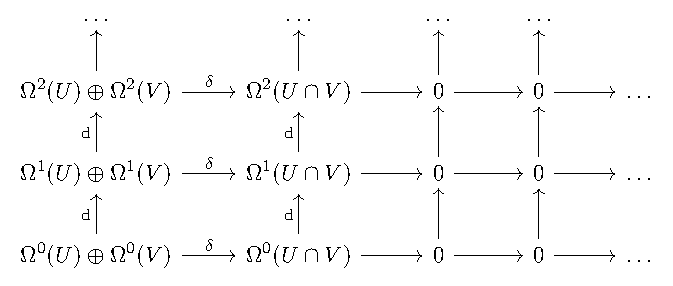
\includegraphics{lectures/7/pictures/cd_30.pdf}
	\end{center}

	Как известно, из биградуированного комплекса всегда можно изготовить его тотализацию суммируя вдоль антидиагоналей
	\[
		K^n \eqdef \bigoplus_{p + q = n} K^{p, q}, \quad K^0 \to K^1 \to \ldots \to K^n \to K^{n + 1},
	\]
	 дифференциал в котором определяется таким образом
	 \[
	 	D = \delta + (-1)^p\mathrm{d} \text{ на } K^{p, q}, \quad D\colon K^n \to K^{n + 1}. 
	 \]

	 Здесь мы для всего этого дела заведём еще такие обозначения (их смысл можно будет понять потом): 
	 \[
	 	C^{\bullet}(\fU, \Omega^{\bullet}) = \bigoplus K^{p, q} = \bigoplus C^{p}(\fU, \Omega^{q}), \quad K^{0, q} = C^{0}(\fU, \Omega^{q}), \quad K^{1, q} = C^{1}(\fU, \Omega^q).
	 \]
	
	 \begin{remark}
	 	В дифференциале $D$ мы альтернируем знак от столбца к столбцу, чтоб он вообще говоря был дифференциалом: 
	 	\[
	 		D^2 = \mathrm{d}^2 \pm \delta \mathrm{d} \mp \mathrm{d}\delta + \delta^2 = 0. 
	 	\]
	 \end{remark}

	 Итак, у нас есть дифференциальный комплекс $(K^{\bullet}, D) = (C^{\bullet}(\fU, \Omega^q), D)$.

	 \begin{theorem} 
	  	Когомологии комплекса $(C^{\bullet}(\fU, \Omega^q), D)$ совпадают с когомологиями де Рама многообразия $M$. 
	  \end{theorem} 
	  \begin{proof}
	  	Рассмотрим отображение сужения 
	  	\[
	  		r\colon \Omega^{\bullet}(M) \to K^{\bullet}, \quad \omega \mapsto (\omega\vert_{U}, \omega_{V}) 	
	  	\]

	  	Во-первых, покажем, что оно индуцирует цепное\footnote{С точностью до знака. На самом деле, ясно, что этого достаточно, так как для вычисления когомологий мы считаем ядра и образы (а они от смены знаков не зависят). } отображение на комплексах. Для этого нужно проверить коммутативность\footnote{с точностю до знака} всех квадратов вот такого вида:
	  	\begin{center}
	  		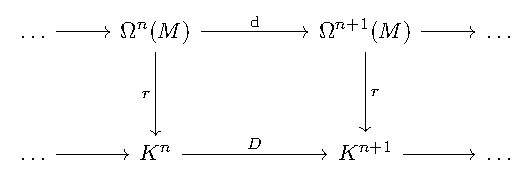
\includegraphics{lectures/7/pictures/cd_31.pdf}
	  	\end{center}
	  	
	  	Для этого заметим, что $\delta r = 0$, так как отображения действуют вот таким образом:
	  	\begin{center}
	  		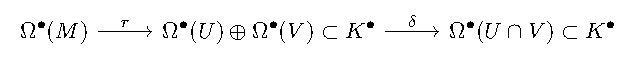
\includegraphics{lectures/7/pictures/cd_32.pdf}
	  	\end{center}
	  	Действительно, $(\omega\vert_{U} - \omega\vert_{V})\vert_{U \cap V} = 0$. 

	  	Тогда мы имеем
	  	\[
	  		Dr = (\delta + (-1)^p\mathrm{d})r = (-1)^p \mathrm{d}r = (-1)^p r \mathrm{d},
	  	\]
	  	что и требовалось. 

	  	Значит, $r$ индуцирует отображение в когомологиях 
	  	\[
	  		r^* \colon H^{\bullet}_{\dR}(M) \to H^{\bullet}\lr*{C^{\bullet}(\fU, \Omega^{\bullet})}. 
	  	\]

	  	Рассмотрим $\alpha \in K^{q}$, тогда она может быть представлена в виде 
	  	\[
	  		\alpha = \alpha_0 + \alpha_1, \quad \text{ где } \alpha_0 \in K^{0, q} = \Omega^{q}(U) \oplus \Omega^{q}(V), \ \alpha_1 \in K^{1, q - 1} = \Omega^{q - 1}(U \cap V).
	  	\]
	  	Вспомним, что последовательность Майера-Виеториса точна: 
	  	\[
	  		0 \to \Omega^{q - 1}(U \cup V) \to \Omega^{q - 1}(U) \oplus \Omega^{q - 1}(V) \xrightarrow{\delta} \Omega^{q - 1}(U \cap V) \to 0,
	  	\]
	  	откуда $\alpha_1 = \delta \beta$ для некоторой $\beta \in \Omega^{q - 1}(U) \oplus \Omega^{q - 1}(V) = K^{0, q - 1}$. Тогда 
	  	\[
	  		\alpha - D\beta = \alpha_0 - \mathrm{d}\beta \in K^{0, q}.
	  	\]
	  	Соотвественно, в комплексе $C^{\bullet}(\fU, \Omega^{\bullet})$ любая коцепь когомологична коцепи с только $(0, q)$-компонентой. 

	  	Теперь докажем, что $r^*$ сюръектвно. Возьмём $[\varphi] \in H^{\bullet}\lr*{C^{\bullet}(\fU, \Omega^{\bullet})}$. По зачмечанию выше, мы можем выбрать представителя когомологического класса так, что он имеет только $(0, q)$ компоненту. Тогда 
	  	\[
	  		0 = D\varphi = (\mathrm{d} + \delta)\varphi = \mathrm{d}\varphi + \delta \varphi \implies \mathrm{d}\varphi = 0,
	  	\]
	  	значит $\varphi$ замкнута и в качестве прообраза нам подойдёт её класс в когомологиях де Рама (от $U \cup V$, а глобальным мы можем его полагать, так как $\delta \varphi = 0$). 

	  	Теперь покажем, что $r^*$ инъективно. Пусть $r^*([\omega]) = 0$, то есть $r^*(\omega) = D\varphi$ для некоторой коцепи $\varphi \in C^{\bullet}(\fU; \Omega^{\bullet})$. Тогда, как мы отмечали, мы можем записать  $\varphi = \varphi' + D\varphi''$, где $\varphi \in K^{0, q}$.  Тогда $r(\omega) = D\varphi' = \mathrm{d}\varphi'$ и $\delta\varphi' = 0$, откуда $\omega$~--- точная форма на $M$. 


	  \end{proof}

	  \subsubsection{Последовательность Майера-Виеториса для счётного покрытия}

	  Пусть $\cJ$~--- счётное упорядоченное индексное множество, $\fU = \{ U_{\alpha} \}_{\alpha \in \cJ}$~-- пассматриваемое нами открытое покрытие многообразия $M$. 

	  Введём такие обозначения для пересечений: 
	  \[
	  	U_{\alpha} \cap U_{\beta} = U_{\alpha \beta}, \quad U_{\alpha} \cap U_{\beta} \cap U_{\gamma} = U_{\alpha \beta \gamma} \text{ и т.д. }
	  \]

	  Тогда у нас есть такая диаграмма: 

	  \begin{center}
	  	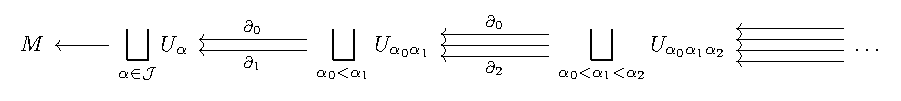
\includegraphics{lectures/7/pictures/cd_33.pdf}
	  \end{center}

	  где отображение $\partial_i$~--- вложение, игнорирующее $i$-е открытое множество, т.е. 
	  \[
	  	\partial_i(U_{\alpha_1 \ldots \alpha_i \ldots \alpha_k}) = U_{\alpha_1 \ldots \widehat{\alpha_i} \ldots \alpha_k}
	  \]
	  Например, $\partial_0(U_{\alpha_0 \alpha_1 \alpha_2}) = U_{\alpha_1 \alpha_2}$ и дальше в том же духе.  Эта последовательность вложений индуцирует последовательность ограничений форм: 

	  \begin{center}
	 		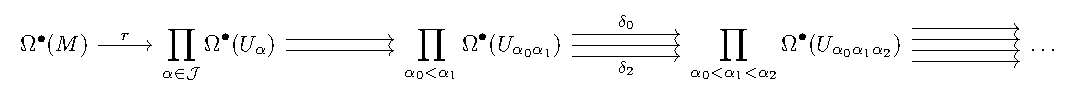
\includegraphics{lectures/7/pictures/cd_34.pdf}
	  \end{center}

	  Немного поясним, как устроены отображения в ней. например, $\delta_0$ индуцированно вложением 
	  \[
	  	\partial_0 \colon \prod_{\alpha} U_{\alpha \beta \gamma} \to U_{\beta \gamma} \rightsquigarrow \delta_0 \Omega^{\bullet}(U_{\beta \gamma}) \to \prod_{\alpha} \Omega^{\bullet}(U_{\alpha \beta \gamma})
	  \]
	  и устроено оно, как сужение. 

	  Определим на этой последовательности оператор разности, который будет действовать 
	  \[
	  	\delta \colon \prod_{\alpha_1 < \ldots < \alpha_p} \Omega^q(U_{ \alpha_0 \ldots \alpha_p}) \to \prod_{\alpha_1 < \ldots < \alpha_{p + 1}} \Omega^q(U_{ \alpha_0 \ldots \alpha_p \alpha_{p + 1}})
	  \]

	  Рассмотрим форму $\omega \in \prod_{\alpha_1 < \ldots < \alpha_p} \Omega^q(U_{ \alpha_0 \ldots \alpha_p}) \to \prod_{\alpha_1 < \ldots < \alpha_{p + 1}}$. Достаточно определить $\delta$ на каждое её компоненте, т.е. сужении $\omega_{\alpha_0 \ldots \alpha_p} \in \Omega^q(U_{ \alpha_0 \ldots \alpha_p}$. Это мы сделаем так: 
	  \[
	  	(\delta \omega)_{\alpha_0 \ldots \alpha_{p + 1}} = \sum_{i = 0}^{p + 1} (-1)^i \omega_{\alpha_0 \ldots \widehat{\alpha_i} \ldots \alpha_{p + 1}}.
	  \]

	  На самом деле, работает это не очень сложно. Например, если у нас есть форма на из $\prod_{\alpha} \Omega^{q}(U_{\alpha})$ то у нас есть по форме на каждом куске покрытия и чтоб изготовить по форме на каждом попарном пересечении мы просто берём все попарные разности. В случае с тройками~--- альтернированные суммы. В общем, нетрудно видеть, что 
	  \[
	  	\delta = \sum_{i} (-1)^i \delta_i.
	  \]

	  \begin{statement} 
	  	$\delta^2 = 0$.
	  \end{statement}
	  \begin{proof}
	  	Действительно, это очевидно, так как мы просто дважды опускаем индексы $\alpha_i $ и $\alpha_j$ и каждый раз с противоположным знаком (так что всё сократится). 
	  \end{proof}

	  \begin{remark}
	 	До этого момента мы полагали, что индексы упорядочены монотонно. Теперь для удобства будем допускать и общий случае, но с таким условием: когда мы меняем два индекса местами, форма меняет знак. 
	 \end{remark}

	 Итак, у нас есть послеовательность 
	 \begin{center}
	 	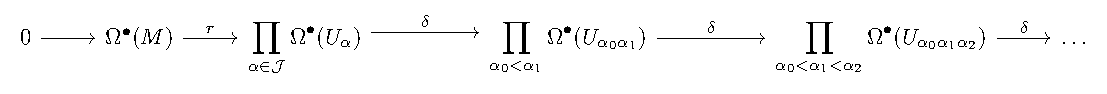
\includegraphics{lectures/7/pictures/cd_35.pdf}
	 \end{center} 

	 

	 Её называют \emph{обобщенной последователньностью} Майера-Виеториса. 

	 \begin{statement} 
	 	Эта последовательность точна.
	 \end{statement}
	 \begin{proof}
	 	
	 	Точность в первом члене очевидна: форма из $\prod_{\alpha} \Omega^{\bullet}(U_{\alpha})$ является глобальной формой на $M$ (т.е.) элементом из $\Omega^{\bullet}(M)$ тогда и только тогда, когда все её компоненты согласованы на попарных пересечениях элементов покрытия. 

	 	Пусть теперь $\{ \rho_{\alpha} \}$~--- разбиение единицы, подчинённое покрытию $\fU$. Рассмотрим коцикл 
	 	\[
	 		\omega \in \prod_{\alpha_0 < \ldots < \alpha_p} \Omega^{\bullet}(U_{\alpha_0 \ldots \alpha_p} )
	 	\]
	 	и покажем, что он является кограницей. Рассмотрим коцепь $\tau$, определённую так:
	 	\[
	 		\tau_{\alpha_0 \ldots \alpha_{p - 1}} = \sum_{\alpha \in \cJ} \rho_{\alpha} \omega_{\alpha \alpha_0 \ldots \alpha_{p - 1}},
	 	\]
	 	тогда мы имеем 
	 	\[
	 		(\delta \tau)_{\alpha_0 \ldots \alpha_p} = \sum_{i} (-1)^i \tau_{\alpha_0 \ldots \widehat{\alpha_i} \ldots \alpha_p} \sum_{i, \alpha} (-1)^i \rho_{\alpha} \omega_{\alpha \alpha_0 \ldots \widehat{\alpha_i} \ldots \alpha_p}.
 	 	\]
 	 	Так как $\omega$~--- это коцикл, 
 	 	\[
 	 		0 = (\delta \omega)_{\alpha \alpha_0 \ldots \alpha_p} = \omega_{\alpha_0 \ldots \alpha_p} + \sum_{i} (-1)^{i + 1} \omega_{\alpha \alpha_0 \ldots \widehat{\alpha_i} \ldots \alpha_p} = 0,
 	 	\]
 	 	откуда мы имеем 
 	 	\[
 	 		(\delta \tau)_{\alpha_0 \ldots \alpha_p} = \sum_{\alpha} \rho_{\alpha} \sum_{i} (-1)^i \omega_{\alpha \alpha_0 \ldots \widehat{\alpha_i} \ldots \alpha_p} = \sum_{\alpha} \rho_{\alpha} \omega_{\alpha_0 \ldots \alpha_p} = \omega_{\alpha_0 \ldots \alpha_p} \cdot \sum_{\alpha} \rho_{\alpha} = \omega_{\alpha_0 \ldots \alpha_p} .
 	 	\]
 	 	Значит, $\omega = \delta \tau$, что нам и требовалось. 

	 	
	 \end{proof}

	 На самом деле, фактически мы построили оператор цепной гомотопии на этом комплексе: 
	 \[
	 	K\omega = \tau, \quad (K\omega)_{\alpha_0 \ldots \alpha_{p - 1}} = \sum_{\alpha} \rho_{\alpha} \omega_{\alpha \alpha_0 \ldots \alpha_{p - 1}}, 
	 \]
	 покажем, что $K \delta + \delta K = \id$. Действительно, легко видеть, что 
	 \[
	 	(\delta K \omega)_{\alpha_0 \ldots \alpha_p} = \sum_{i}(-1)^k (K\omega)_{\alpha_0 \ldots \widehat{\alpha_i} \ldots \alpha_p} = \sum_{i} (-1)^i \omega_{\alpha \alpha_0 \ldots \widehat{\alpha_i} \ldots \alpha_p}
	 \]
	 \[
	 	(K \delta \omega)_{\alpha_0 \ldots \alpha_p} = \sum_{\alpha} \rho_{\alpha} (\delta \omega)_{\alpha \alpha_0 \ldots \alpha_p} = \omega_{\alpha_0 \ldots \alpha_p} \cdot \sum_{\alpha} \rho_{\alpha} + \sum (-1)^{i + 1} \rho_{\alpha} \omega_{\alpha \alpha_0 \ldots \widehat{\alpha_i} \ldots \alpha_p} = \omega_{\alpha_0 \ldots \alpha_p} - (\delta K \omega)_{\alpha_0 \ldots \alpha_p}.
	 \]

	 Соответственно, так как на нашем комплексе есть оператр стягивающей гомотопии, когомологии комплекса тривиальны. 

	 Как и в случае двуэлементного покрытия, мы можем интерпретировать эту последовательность в виде бикомплекса $(K^{p, q}, \delta, \mathrm{d})$:

	 \begin{center}
	 	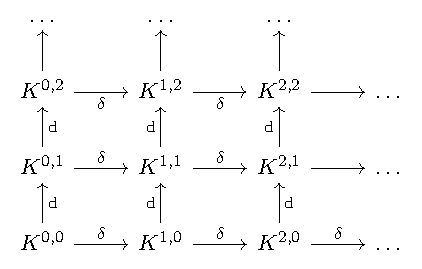
\includegraphics{lectures/7/pictures/cd_36.pdf}
	 \end{center}
	 Или, если рисовать в расширенном виде (добавляя $-1$-й столбец):

	 \begin{center}
	 	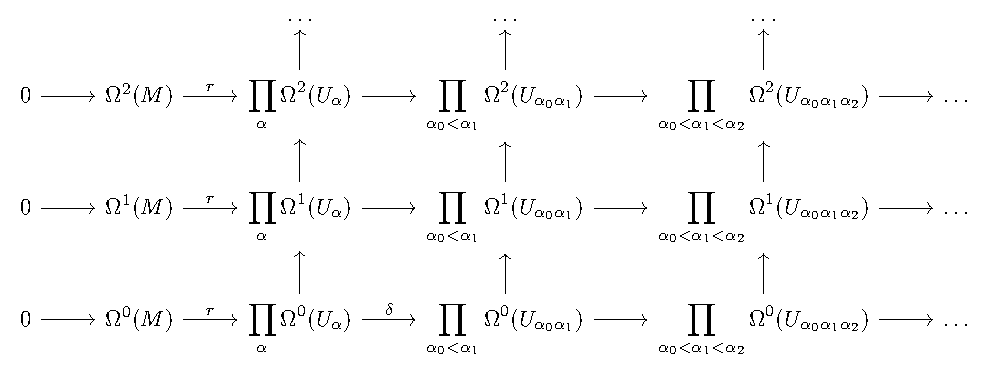
\includegraphics{lectures/7/pictures/cd_37.pdf}
	 \end{center}

	 Соответственно, мы можем ввести такие же как и для покрытия двух множеств обозначения 
	 \[
	 	K^{p, q} = C^{p}(\fU, \Omega^{q}) = \prod_{\alpha_1 < \ldots < \alpha_p} \Omega^q(U_{\alpha_0 \ldots \alpha_p}).
	 \]

	 Соответственно, комплекс $C^{\bullet}(\fU, \Omega^{\bullet})$ называют \emph{комплексом Чеха-де-Рама} и говорят, что $C^{p}(\fU, \Omega^{q})$~--- это $p$-коцепи со значениями в $q$-формах. 

	 Как и всегда, можно рассмотреть его тотализацю
	 \[
	 	(K^{\bullet}, D), \quad K^{n} = \bigoplus_{p + q = n} K^{p, q}, \quad D = \delta + (-1)^p \mathrm{d}.  
	 \]
	 \begin{statement}[Обобщенный принцип Майера-Виеториса]\label{gen_mayer_vietoris_principle} 
	 	Отображение $r\colon \Omega^{\bullet}(M) \to C^{\bullet}(M)$ индуцирует изоморфизм на когомологиях
	 	\[
	 	  	H^{\bullet}_{\dR}(M) \cong H^{\bullet}(C^{\bullet}(\fU, \Omega^{\bullet})).
	 	  \]  
	 \end{statement}

	 \begin{proof}
	 	Доказательство тут аналогично доказательству в случае покрытия из двух множеств. А именно, рассматривая $D$-коцикл $\varphi \in K^n$ мы представляем её суммой 
	 	\[
	 		\varphi = \alpha_0 + \alpha_1 + \ldots + \alpha_n, \quad \alpha_0 \in K^{0, n}, \alpha_1 \in K^{1, n - 1}, \ldots, \alpha_m \in K^{n, 0}.
	 	\]
	 	Пользуясь точностью строк мы поочередно можем убивать компоненты меньше размерности, а именно, в силу точности нижней строчки диаграммы $\alpha_n = \delta \alpha_n'$, где $\alpha_n' \in K^{n - 1, 1}$. Тогда если мы рассмотрим $\varphi - D\alpha_n'$, мы останемся в том же когомологическом классе, но получим коцикл без $K^{n, 0}$ компоненты. Проделывая так достаточное количество раз мы получим коцикл $\widetilde{\varphi}$ только с $K^{n, 0}$ компонентой, оставаясь в том же когомологическом классе. Тогда он будет глобальной замкнутой формой, так как $\mathrm{d}\widetilde{\varphi} = 0, \ \delta\widetilde{\varphi} = 0$ и он из $K^{n, 0}$. 

	 	Аналогично доказывается и инъективность. 
	 \end{proof}

	 На самом деле видно, что мы доказали несколько более общее утверждение: \emph{если строки расширенного двойного комплекса точны, то его $D$-когомологии изоморфны когомологиям начального (-1-го) столбца}. 


	 Теперь добавим к каждому столбцу снизу ядро нижнего дифференциала $\mathrm{d}$, которое мы обозначим как $C^{\bullet}(\fU, \R)$. Как видно из такого определения, $C^{p}(\fU, \R)$ состоит из локально-постоянных функций на $(p+1)$-кратных пересечениях $U_{\alpha_0 \ldots \alpha_p}$.

	 \begin{center}
	 	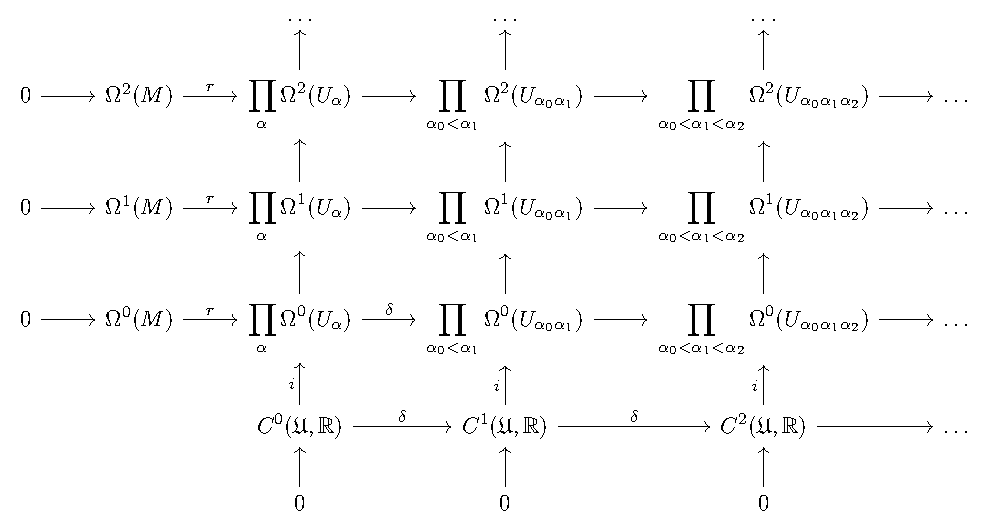
\includegraphics{lectures/7/pictures/cd_38.pdf}
	 \end{center}

	 \begin{definition} 
	 	Соотвественно, построенная только что нижняя часть также является дифференциальным комплексом 
	 \[
	 	C^{0}(\fU; \R) \xrightarrow{\delta} C^{1}(\fU; \R) \xrightarrow{\delta} C^{2}(\fU; \R)  \to \ldots,
	 \]
	 который называется \emph{комплексом Чеха} покрытия $\fU$, а его когомологии, соотвественно, называются \emph{когомологиями Чеха} покрытия $\fU$. Обозначать их мы будем как $H^{\bullet}(\fU, \R)$. 

	 \end{definition}

	 
	 Теперь  заметим, что если и столбцы расширенного комплекса точны, то "поворотом на $\pi/2$" доказательства предложения~\ref{gen_mayer_vietoris_principle} мы получаем, что
	 \[
	  	H^{\bullet}(\fU; \R) \cong H^{\bullet}(C^{\bullet}(\fU, \Omega^{\bullet})) \cong H^{\bullet}_{\dR}(M).
	  \] 

	  Ясно, что столбцы точны совсем не всегда, а препятствие к точности измеряется группами 
	  \[
	  	\prod_{q \ge 1, \ \alpha_0 \le \ldots \alpha_p} H^{q}(U_{\alpha_0 \ldots \alpha_p}).
	  \]
	  Теперь ясно, какое условие нужно требовать: 

	  \begin{definition} 
	  	Назовём покрытие $\fU = \{ U_{\alpha} \}_{\alpha}$ \emph{хорошим}, если все его конечные непустые пересечения стягиваемы. 
	  \end{definition}

	  Таким образом, имеем вот такую теорему: 

	  \begin{theorem} 
	  		Предположим, что многообразие $M$ обладает хорошим покрытием  $\fU$. Тогда $H^{\bullet}_{\dR}(M) \cong H^{\bullet}(\fU; \R)$.
	  \end{theorem}

	  Сделаем теперь несколько забавных наблюдений: можно заметить, что в комплексе Чеха-де-Рама $C^{\bullet}(\fU, \Omega^{q})$ мы <<смешали>> дифференциальную геометрию форм и комбинаторику покрытий. Так вот, из полученного изоморфизма $H^{\bullet}_{\dR}(M) \cong H^{\bullet}(\fU; \R)$ можно делать вот такие интересные выводы: 

	  \begin{itemize}
	  	\item Так как при смене хорошего покрытия когомологии де Рама не изменяются, не изменяются и когомологии Чеха (что вообще говооря совсем не очевидно!). 

	  	\item Так как компактное многообразие допускает конечное хорошее покрытие, а когомологии Чеха такого покрытия конечномерны (по очевидным причинам), конечномерны и когомологии Де Рама (что, как мы видели, вообще говоря. не очевидно). 
	  \end{itemize}







 	  







